% define \title (only used by writelatex.com)
%\title{CSEC-793 Project Report_Blank}
%%%%%%%%%%%%%%%%%%%%%%%%%%%%%%%%%%%%%%%%%%%%%%%%%%%%%%%%%%%%%%%%%%%%%%
% LaTeX Template: Project Titlepage
%
% Source: http://www.howtotex.com
% Date: April 2011
% 
% This is a title page template which be used for articles & reports.
% 
% Feel free to distribute this example, but please keep the referral
% to howtotex.com
% 
%%%%%%%%%%%%%%%%%%%%%%%%%%%%%%%%%%%%%%%%%%%%%%%%%%%%%%%%%%%%%%%%%%%%%%
% How to use writeLaTeX: 
%
% You edit the source code here on the left, and the preview on the
% right shows you the result within a few seconds.
%
% Bookmark this page and share the URL with your co-authors. They can
% edit at the same time!
%
% You can upload figures, bibliographies, custom classes and
% styles using the files menu.
%
% If you're new to LaTeX, the wikibook is a great place to start:
% http://en.wikibooks.org/wiki/LaTeX
%
%%%%%%%%%%%%%%%%%%%%%%%%%%%%%%%%%%%%%%%%%%%%%%%%%%%%%%%%%%%%%%%%%%%%%%
%
% --------------------------------------------------------------------
% Preamble
% --------------------------------------------------------------------
\documentclass[ fontsize=11pt,twoside]{scrartcl}	% KOMA

\usepackage[letterpaper,pdftex]{geometry}	% A4paper margins
\setlength{\oddsidemargin}{5mm}			% Remove 'twosided' indentation
\setlength{\evensidemargin}{5mm}

\usepackage[english]{babel}
\usepackage[protrusion=true,expansion=true]{microtype}	
\usepackage{amsmath,amsfonts,amsthm,amssymb}
\usepackage{graphicx}
\usepackage{pseudocode}

\usepackage[latin1]{inputenc}
\usepackage{tikz}
\usetikzlibrary{shapes,arrows}


% --------------------------------------------------------------------
% Definitions (do not change this)
% --------------------------------------------------------------------
\newcommand{\HRule}[1]{\rule{\linewidth}{#1}} 	% Horizontal rule

\makeatletter							% Title
\def\printtitle{%						
    {\centering \@title\par}}
\makeatother									

\makeatletter							% Author
\def\printauthor{%					
    {\centering \Large \@author}}				
\makeatother							

% --------------------------------------------------------------------
% Metadata (Change this)
% --------------------------------------------------------------------
\title{	\Large \textsc{ CSEC 793 Capstone in Computing Security \\ 
															Project Report} 	% Subtitle
		 	\\[2.0cm]								% 2cm spacing
			\HRule{2pt} \\						% Upper rule
			\LARGE \textbf{\uppercase{This is my MS capstone report}}	% Title
			\HRule{2pt} \\ [0.5cm]		% Lower rule + 0.5cm spacing
			\Large \today			% Todays date
		}

 \author{
		Sumita Mishra\\	
		Department of Computing Security\\	
        College of Computing and Information Sciences \\
		Rochester Institute of Technology\\
        \texttt{sumita.mishra@rit.edu} \\
}


\begin{document}
% ------------------------------------------------------------------------------
% Maketitle
% ------------------------------------------------------------------------------
\thispagestyle{empty}		% Remove page numbering on this page

\printtitle					% Print the title data as defined above
  	\vfill
\printauthor				% Print the author data as defined above
\newpage
% ------------------------------------------------------------------------------
% Begin document
% ------------------------------------------------------------------------------
\setcounter{page}{1}		% Set page numbering to begin on this page


%%%%%%%%%%%%%%%
%														%
% 			Main Contents            %
%														%
%%%%%%%%%%%%%%%

\section{Abstract}

This section provides on overview about the project. It should be completed at the very last stage of the writing, i.e., after you have completed all the other sections.  
\section{Introduction}
    The objective of this paper is the development of a security focused continuous integration (CI) pipeline. The goal is to make a pipeline that focuses on security in an attempt to improve web
    application security. This pipeline will automatically run a series of tests against a repository of configuration files and code. These tests will enforce correct configurations and security
    best practices within committed changes.

    CI is a technique that is used to speed up development releases by ensuring code changes do not break the existing code base. Those benefits can also be tailored to improve security in 
    development. Many penetration tests or bug reports revolve around the same information repeated for different cases. These reports often have a common solution. If we discuss web applications, one 
    common vulnerability is cross site scripting (XSS). XSS vulnerabilities have the short term recommendation of encoding all user input to avoid users input being interpreted as part of the webpage. 
    The long term recommendation is to set up a full Content Security Policy (CSP), limiting where scripts and HTML tags can be loaded from. Companies generally choose the short term route of fixing 
    each individual case, but this will cost them too much time and money in the long term, eventually leading them to implement a long term solution. In this example companies will often implement encoding, 
    but as they expand the web application, they find the same bug. The company eventually switches to creating a CSP and configuring it correctly so new expansions can not be affected by a XSS bug.
    
    Everyday applications are getting larger and are handling enormous amounts of data. Many of these applications are services that companies provide, such as Facebook and Netflix. All of these 
    applications need to provide security for both their internal company data and the end user's data. The problem is that as these applications grow, their logic gets more complex and mistakes will 
    be made, potentially introducing vulnerabilities into the codebase without the developers realizing until it is too late. Sometimes these mistakes are simply forgotten flags on cookies and other
    times they can be complex flaws in the business logic of the application. These mistakes can result in damage ranging from defacement of a company site, to a complete breach of a company's 
    internal network.

	A bug does not need to be exploited by a malicious actor to cause financial loss for the company. Many companies offer bug bounty programs, in which a researcher can discover and report a bug 
    for a reward. The rewards vary by company, but often times the researcher will receive a substantial monetary reward, depending on the severity of the bug discovered. This means that each time 
    the company releases updates to their applications, researchers will be scavenging for more vulnerabilities, which can be costly for the company. It may also cost the company's security team a 
    significant amount of time, as they need to look into and verify each report that is submitted. Often times, researchers can find very common vulnerabilities in the application, that usually 
    result from developers rushing to push out new features at such a rapid pace.

	CI can be used to catch simple mistakes automatically, by ensuring that the common bugs are found before the changes are deployed into production. By discovering these bugs before they are introduced 
    into production, the number of submissions from bug bounty programs will decrease dramatically. This is beneficial to the company as it reduces the number of simple submissions, saving the business
    time and money, while the bug reports that are submitted provide more value to the company.

    This paper shows that the development and application of security tests into CI uses the same methods as normal unit testing. The main difference between normal unit testing and security testing
    is that security testing does not focus on the specific functionality of an application, but instead on the testing of generalized security controls. For these tests it is found that dynamic
    tests are more appropriate than static because they can then span accross multiple languages. Further the usefullness of containerization is enforced by how it simplifies dynamic testing in a CI
    pipeline.

\section{Literature Review}

\subsection{Introduction}
    Continuous Integration (CI) has grown in popularity, being used in both enterprise and open source projects. CI provides an increase in productivity to programming projects by creating an 
    environment where building, testing, and often deployment is done automatically. When developers do not need to do these tasks manually they can spend more time programming and finding bugs that 
    trigger a failed build or failed test. Most research into CI looks at increasing productivity of developers and the enforcement of development standards. The potential use of CI for security has 
    been mostly overlooked with most research looking at exploiting and protecting a CI system or a CI pipeline and not at the benefits of a pipeline focusing on application security.

	A separate pipeline for security could provide a number of benefits for a security baseline. It could force certain configurations such as Content Security Policy in web applications, or lack of 
    use of depreciated crypto algorithms such as DES or TripleDES \cite{Vehent}. A pipeline that looks only at big win configurations such as these would serve a similar function as Automated Source 
    Code Analysis Tools (ASCAT) do when looking at code meeting project coding guidelines \cite{Zampetti}. The pipeline could also include ASCATs that search for security bugs in a warning stage to 
    avoid wasted time with failed builds from false positive. Another potential feature is an inclusion of fuzzers, which were recently used against memory forensic tools to look into anti-forensics 
    techniques through crashing the tools \cite{Case}.

\subsection{Test case generation}
    Test case generation is a discipline that focuses around automatically generate unit tests for Software Engineering projects. The discipline sometimes focuses on generating tests from a base,
    such as the source code or a config file, and generating a set of tests from the base or it focuses on taking existing tests and exanpding them to cover more features.

    One paper from the 2014 Automated Software Engineering conference looked at generating test cases for web from an existing selenium test suite \cite{WebTestGeneration}. 
    This paper goes through the method that is used to generate the new test cases. The method starts by taking a selenium test suite and going though it keeping track of states, 
    http element interactions, and test case assertions. It uses the base states and element interactions to create a State-Flow Graph, which is a graph of the states with the interations 
    that that move from one state to the next and the assertions that are involved to a single state. It then uses a web crawler on each state to discover alternate paths and new states. 
    It then makes use of assertions on the base states to generate new tests for the crawler discovered states. An example given in the paper is that an application that allows you to 
    create notes is tested with selenium by logging in, clicking the create note element, and then verifiying that an id element had specific text. The test suite was then expanded by crawling
    to find the edit note interaction and the delete note interaction. These were then clicked and tested using the assertion, verifying that the id was present and changing the text to match the
    new interactions result text.

\subsection{Test case selection}
    The idea behind test case selection is limiting tests run to save on time during builds. As a code base grows, the number of tests increase. The increase in tests make it more and more expensive
    and eventually becomes to big a load to do everytime \cite{googletest, googlescale}. This has lead to ways of avoiding running all of the tests on every code change. The ways of running tests
    have historically been either rerun all of the tests or manually pick test cases to run based off of the changes the developer made.

    A paper by Milos Gligoric looks at comparing manual test selection against research made into automatic test selection, where automatic test selection would only run the tests that test code
    affected by the changes a developer made \cite{TestCaseSelction}. The state of the automatic test selection tools were limited to Google and Microsoft at the time of the paper. The tools were
    impractical for use by smaller projects because they were either too imprecise, selected tests that were not affected by the code changes, or unsafe, failed to guarentee all tests not selected
    were unaffected by the code changes. The paper specifically compares 14 developers manual test choices against a tools automated test selection. The paper found that manual test case selection
    was most commonly done during debugging. It also found the 73\% of the time manual RTS selected more tests than were necessary and 74\% of the time some tests that were affected were missed.

\subsection{Effective use of CI}
	Continuous integration has been a fantastic addition to Software Engineering practices by removing repetitive administrative tasks. The less steps a software engineer has to go through when 
    producing new code, the more time they can spend on adding features, squashing bugs, or otherwise improving the project code base. There is plenty of research done into the use of CI 
    including many case studies, papers and presentations looking at how to setup CI and Continuous Deployment (CD), and papers looking at specific configurations of CI.
	
	CI can be integrated with all sorts of tools to increase productivity. The paper How Open Source Projects use Static Code Analysis Tools in Continuous Integration Pipelines by Fiorella Zampett 
    looks at how Static Code Analysis tools in a CI pipeline effects projects \cite{Zampetti}. The paper found that the most utilized feature of ASCATs was to ensure a project's code was consistent 
    by ensuring the developers coding guidelines were met. The paper also found that ASCATs caused broken builds to be fixed quickly in an average of 8 hours and one build. There are a number of 
    recommendations that this paper provides which outline how to set up ASCATs in a CI pipeline, what to think about when doing so, and what to expect to maintain the ASCAT. Adding a source code 
    analysis tool will help keep a project consistent while helping point out bugs that could be missed by developer made unit tests.

	Two papers look at CI and how it affects projects in general. Continuous Integration and Quality Assurance: A Case Study of Two Open Source Projects by Jesper Holck and Usage, Costs, and Benefits
    of Continuous Integration in Open-Source Projects by Michael Hilton both look at open source projects and how CI affects them \cite{Hilton,Holck}. The papers found that CI often replaces the 
    practice of having developers make formal design documents. The developers instead just pick from a list of tasks and works on completing them and merging them into the code base. The papers also
    found that most developers like CI and plan to use it again in future projects. For projects that did not use CI it was found that the reason was usually just that the developers were not 
    familiar with how to set up and use CI. Both papers found CI to be successful in increasing productivity, causing projects to release twice as often, accept pull requests quicker, and have 
    developers less worried about breaking the project. 

\subsection{Security in CI pipelines}
	Security conferences often look into how to break systems as a way of pointing out the flaws of a configuration. CI servers have also had their share of security professionals testing for exploits
    and looking at the consequences of compromise. CI has also had a little bit of research into how to secure a CI pipeline.

	A presentation at DEFCON named Exploiting Continuous Integration (CI) and Automated Build Systems talked about the consequences of a CI enabled projects \cite{spaceb0x}. The presentation found that 
    exploiting a repo that holds a CI integration ends with a huge amount of access. If the repo links into an internal CI server, then the attacker ends up with internal network access. If the repo 
    links to a CI server with multiple CI instances or also runs the CD, then the attacker will get more source code and access to the deployment machines because the CI holds a way to connect to the 
    deployment servers. Otherwise the attacker ends up with environment variables which often hold extremely sensitive information.

	A paper by Len Bass called Securing a Deployment Pipeline looks at how to secure a CI pipeline to limit the damage in case of exploitation \cite{Bass}. The paper details a way to break a pipeline 
    down into trusted and untrustworthy parts, segmenting operations until an untrustworthy segment cannot be broken down any more. The CI pipeline then holds parts that are guaranteed to be 
    trustworthy and run as expected, minus specific cases outlined in the paper, and parts that may provide untrustworthy output. By limiting the scope of untrustworthy parts, the rest of the pipeline
    can run as expected and it is possible to see where the most risk lies. Then the owners of the pipeline can work to limit access to the untrustworthy portions and look into solutions to make those
    portions trustworthy.

\subsection{Use of CI for Security}
    There is little research into the use of CI for security. One presentation by Mozilla looks at the use of CI to tackle easy fixes in response to their bug bounty program \cite{Vehent}. The 
    presentation looks at using CI to ensure that the production environment contains configurations that mirror best practices for common web application security bugs. Some examples include HSTS
    is enabled, CSP for XSS bugs, various X-OPTIONS headers, Cookies have secure, Cross origin sharing, and Subresource integrity checks. The presentation recommends figuring out a security baseline
    for a projects CI pipeline, drive testing from the CI pipeline, and empower the team to fix the issues. Another recommendation is not to break on deployment into production as that could break the
    production site if configured poorly. The end result of mozilla's CI setup was a large drop in bug reports that the CI tests aimed to fix.

\section{Work and methodology}
	The work into CI so far has shown that CI is useful tool for developers to ease the creation of new features. CI has spread to open source projects and is deployed in most organizations that have 
    at least one large code project. The security side of how a CI is dangerous if exploited and how to secure a pipeline against attacks has had little research. The most interesting thing that I 
    think is lacking is the look into how CI can be used to improve the security the project that it is integrated on.
	
	Most of the research does not mention how CI could help improve the security of a project. Some ways this could be done are through targeting common bugs that are already fixed. Some examples
    are ensuring that CSP is enabled, HSTS is enabled, parameterized queries are used, binary protections are enabled in compilation scripts, and unsafe functions are not used. Some of these are
    implemented already in some source code analysis tools, but these tools often have high levels of false positives. Another use could be in including fuzzing in a pipeline. I have not seen any
    research into automating fuzzing into testing an application. Depending on the project it could be a very useful tool to find bugs.

    The research I am doing involves creating a pipeline with tests that focus on specific frameworks and are tailored towards an application instead of general language based tests. Most source
    code analysis tools look at specific languages instead of focusing on specific libraries or frameworks \cite{bandit, findbugs, findsecbugs}. My tests will also do some dynamic testing
    instead of just focusing on source code analysis to verify that the protections are in place in a live application. I am following a similiar path to Mozilla in using tests to mandate security
    configurations \cite{Vehent}.

\section{Your project idea}

In this section, first  redefine the problem in great details. Then describe your solutions. Try to use as many illustrations such as pictures, graphs, pseudo code as you see fit. Here are some examples of including pictures, graphs, and pseudo code in latex. 

%%%%%%%%%%%%%%%%%%%%%%%%%%%%%%%%%%%%%%%%%%%%%%%%%%%%%%%%%%%%%%%%%%%
%
% Commands to include a figure:
%
%%%%%%%%%%%%%%%%%%%%%%%%%%%%%%%%%%%%%%%%%%%%%%%%%%%%%%%%%%%%%%%%%%%
Figure~\ref{fig:fig1} shows how to include a picture in a Latex document. 
\begin{figure}[!ht]
 \centering

\includegraphics[width=3in]{sample_1}
\caption{\label{fig:fig1}This is my great security design.}
\end{figure}

%%%%%%%%%%%%%%%%%%%%%%%%%%%%%%%%%%%%%%%%%%%%%%%%%%%%%%%%%%%%%%%%%%%
%
% The following pseudo code is copied from 
% http://users.sdsc.edu/~ssmallen/latex/pseudocode.html
%
%%%%%%%%%%%%%%%%%%%%%%%%%%%%%%%%%%%%%%%%%%%%%%%%%%%%%%%%%%%%%%%%%%%
Figure~\ref{fig:fig2} is a sample pseudo code copied from this site \cite{pseudocode}. 

\begin{figure}[!ht]
 \centering

  \begin{pseudocode}[framebox]{reduce}{projection, x, y, f}
    \FOR i \GETS 1 \TO y/f \DO
      \BEGIN
      \FOR j \GETS 1 \TO x/f \DO
        \BEGIN
        sum \GETS 0 \\
        \FOR m \GETS 1 \TO f \DO
          \BEGIN
          \FOR n \GETS 1 \TO f \DO
            sum = sum + projection[i*f+m][j * f+n]  \\
          \END \\
        reducedProjection[i][j] = sum / (f * f) \\
        \END
      \END \\
  \RETURN{reducedProjection}
  \end{pseudocode}
  
  \caption{\label{fig:fig2}This is my great pseudo code}
  
  \end{figure}
  
%%%%%%%%%%%%%%%%%%%%%%%%%%%%%%%%%%%%%%%%%%%%%%%%%%%%%%%%%%%%%%%%%%%
%
% Latex float chart example
% Copied from http://www.texample.net/tikz/examples/simple-flow-chart/
%
%%%%%%%%%%%%%%%%%%%%%%%%%%%%%%%%%%%%%%%%%%%%%%%%%%%%%%%%%%%%%%%%%%%

Figure~\ref{fig:fig3} is a sample float chart is copied from this website \cite{floatchart}

\tikzstyle{decision} = [diamond, draw, fill=blue!20, 
    text width=4.5em, text badly centered, node distance=3cm, inner sep=0pt]
\tikzstyle{block} = [rectangle, draw, fill=blue!20, 
    text width=5em, text centered, rounded corners, minimum height=4em]
\tikzstyle{line} = [draw, -latex']
\tikzstyle{cloud} = [draw, ellipse,fill=red!20, node distance=3cm,
    minimum height=2em]
   
  \begin{figure}[!ht]
 \centering
 
\begin{tikzpicture}[node distance = 2cm, auto]
    % Place nodes
    \node [block] (init) {initialize model};
    \node [cloud, left of=init] (expert) {expert};
    \node [cloud, right of=init] (system) {system};
    \node [block, below of=init] (identify) {identify candidate models};
    \node [block, below of=identify] (evaluate) {evaluate candidate models};
    \node [block, left of=evaluate, node distance=3cm] (update) {update model};
    \node [decision, below of=evaluate] (decide) {is best candidate better?};
    \node [block, below of=decide, node distance=3cm] (stop) {stop};
    % Draw edges
    \path [line] (init) -- (identify);
    \path [line] (identify) -- (evaluate);
    \path [line] (evaluate) -- (decide);
    \path [line] (decide) -| node [near start] {yes} (update);
    \path [line] (update) |- (identify);
    \path [line] (decide) -- node {no}(stop);
    \path [line,dashed] (expert) -- (init);
    \path [line,dashed] (system) -- (init);
    \path [line,dashed] (system) |- (evaluate);
\end{tikzpicture}

  \caption{\label{fig:fig3}This is my great float chart}
  
  \end{figure}


%%%%%%%%%%%%%%%%%%%%%%%%%%%%%%%%%%%%%%%%%%%%%%%%%%%%%%%%%%%%%%%%%%%

\subsection{Mathematics}

If your project idea needs mathematics to formulate your methods, \LaTeX{} is great at typesetting mathematics. Let $X_1, X_2, \ldots, X_n$ be a sequence of independent and identically distributed random variables with $\text{E}[X_i] = \mu$ and $\text{Var}[X_i] = \sigma^2 < \infty$, and let
$$S_n = \frac{X_1 + X_2 + \cdots + X_n}{n}
      = \frac{1}{n}\sum_{i}^{n} X_i$$
denote their mean. Then as $n$ approaches infinity, the random variables $\sqrt{n}(S_n - \mu)$ converge in distribution to a normal $\mathcal{N}(0, \sigma^2)$.

\section{Project Implementation}
The project's goal is a way to mandate security with low false positives. The start of this project involved creating a list of checks to implement as shown in Figure~\ref{fig:fig1}.
\begin{figure}[!ht]
  \centering
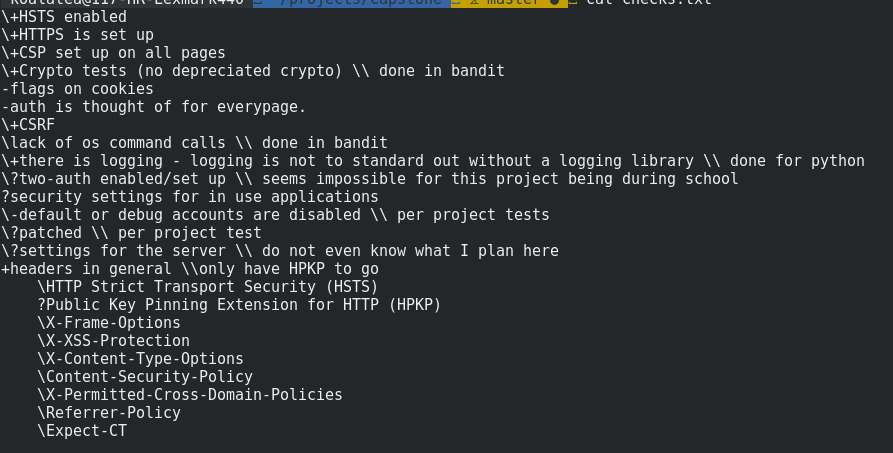
\includegraphics[width=4in]{unittestchecks}
\caption{\label{fig:fig1}}The list of checks to implement
\end{figure}
The checks were chosen for both their ease of being checked and their security relevance. Tests that could be dynamic were prioritized over those that had to be static. The notation in 
Figure~\ref{fig:fig1} checks is that a leading $\backslash$ means the test is addressed, a + means that the test has been chosen to be implemented, a - meant the test would not be implemented, and a ?
meant that there are still questions about the test. The majority of tests implemented are headers, with each one making specific bugs harder to exploit.

The implemented tests were all of the headers tests, and the logging test. The depreciated crypto test and the os test were both found to be done for python in the bandit source code analysis tools
\cite{bandit}. The HPKP header was dropped due to it's pending removal from chrome in favor of the new Expect-CT header \cite{hpkp}. The headers are chosen because they are easy to test for
dynamically, the same rationale applies to csrf and https. The only static test that is created for this project is the logging test one because it does not require context like authentication being
addressed for every web page. Figure~\ref{fig:fig2} shows failing dynamic tests and Figure~\ref{fig:fig3} shows passing dynamic tests. At the top of Figure~\ref{fig:fig3} 12 dots can be seen these
represent the result of the tests in a failed case the . will instead be an F and if the test errors it will be an E.
\begin{figure}[!ht]
  \centering
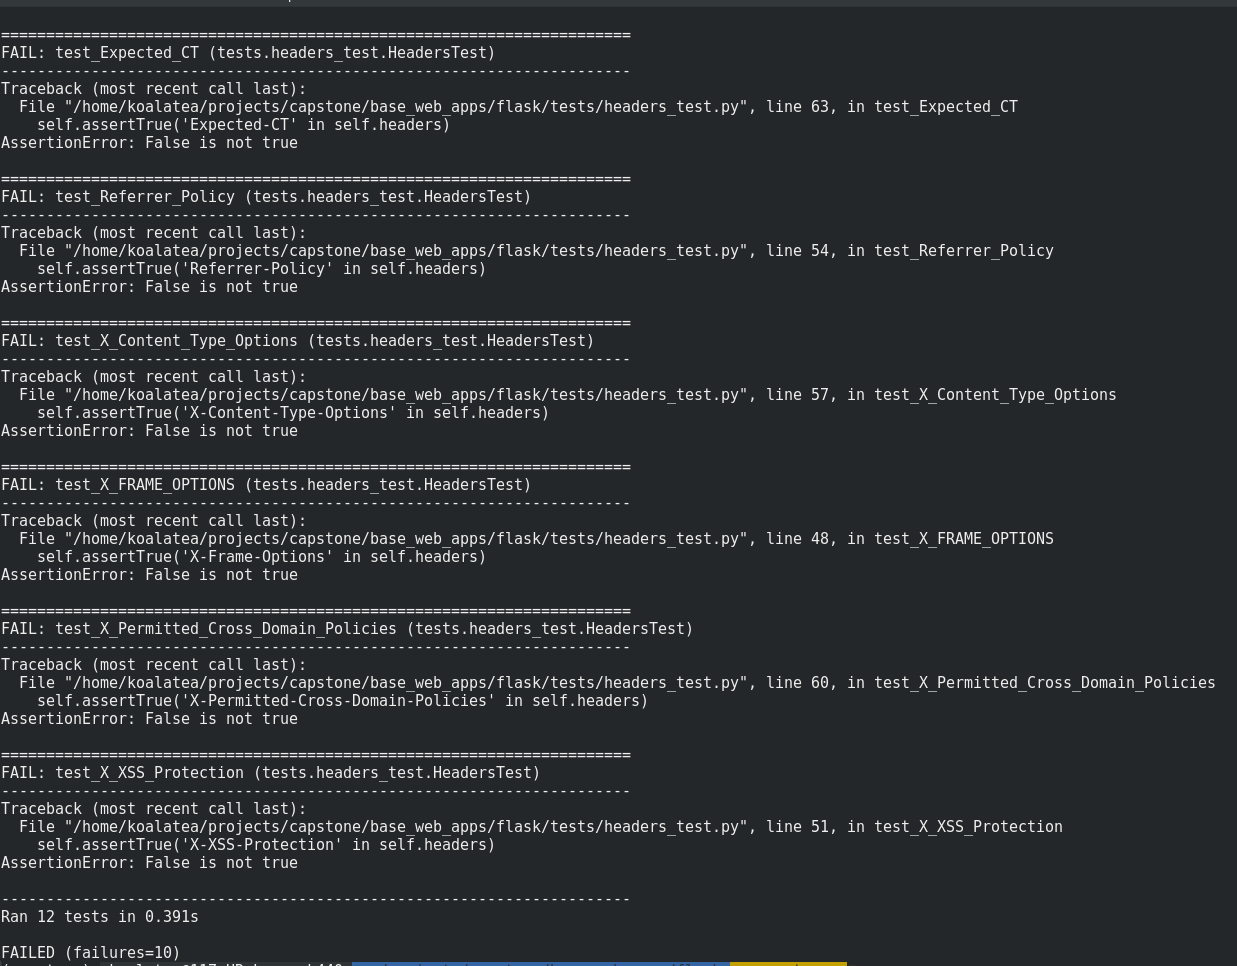
\includegraphics[width=5in]{unittestfail}
\caption{\label{fig:fig2}}Example execution of failing tests
\end{figure}
\begin{figure}[!ht]
  \centering
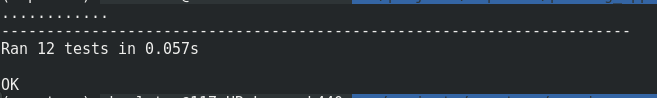
\includegraphics[width=4in]{unittestpass}
\caption{\label{fig:fig3}}Example execution of passing tests
\end{figure}

The HTTPS test is tested by verifying that browsing to HTTP root redirects to an HTTPS root and then that doing a GET request against the HTTPS root returns a 200 response. Following the HTTPS test,
HSTS is tested next by checking the Strict-Transport-Security header and that at least max-age is set, further parts could be included if the developer also wanted includeSubDomains or preload. CSP
is tested in a similar way by checking that the Content-Security-Policy header is present and does not have unsafe-inline within any of the Content-Security-Policy headers. The rest of the headers
are implemented soley by checking for their existence. The headers have settings that are too different between projects so they are not tested for. The CSRF test is implemented using a list of
dictionaries to keep track of end points. Each dictionary is of an endpoint that has a form to fill. The dictionaries have the endpoint, data to post, fail$\textunderscore$text which is the text
present if the form submission failed, success$\textunderscore$text which is the text present if the form submission succeeds, a fail$\textunderscore$status$\textunderscore$code which is the status
code for a failed submission, and a success$\textunderscore$status$\textunderscore$code if the submission succeeds. In the case of there not being one of the four success or fail codes or text then
they are set to none. In the CSRF test for each endpoint the endpoint is queried and is searched for an input html tag with an id of csrf$\textunderscore$token. If the csrf$\textunderscore$token
exists the endpoint is POSTed to without the token. The response to this post is checked for each fail condition that is not none, and reach success condition that is not none is checked to make sure
they are absent. Finally the csrf$\textunderscore$token found earlier is added to the data and POSTed again with the checks from the POST without the token are reversed. The rest of the tests are
static tests. Only one was implemented because it was found that the rest of the planned ones were already implemented. The os tests are done for potential inject points using os, which is slightly
different from the original goal in the checks list, but the crypto one does exactly what is being looked for by checking for depreciated crypto. The written test was written as a plugin for bandit,
it checks for any print statements and recommends using a logging library instead. This one exists partially because most developers already use logging libraries for most projects, the other reason
is for propper logging management to avoid resource exhaustion.

All of the dynamic tests were easy to transfer over to java, only the url and the requests library had to be changed and the test functioned that same. The caveat is that the java application had to
be dockerized so that it could be tested with the python code, while the python tests worked by using flasks built in debug client. The static tests are not as easy to transfer over. To use the
static test the already implemented tests either needed to be found in another static code analysis tool or writen again for java.

These tests were then added to a CI pipeline in Travis. To do so build stages were used for parallelizing the tests. In this project this made sense because there were two passing and two failing
builds. Figure~\ref{fig:fig4} is the travis.yml configuration file.
\begin{figure}[!ht]
  \centering
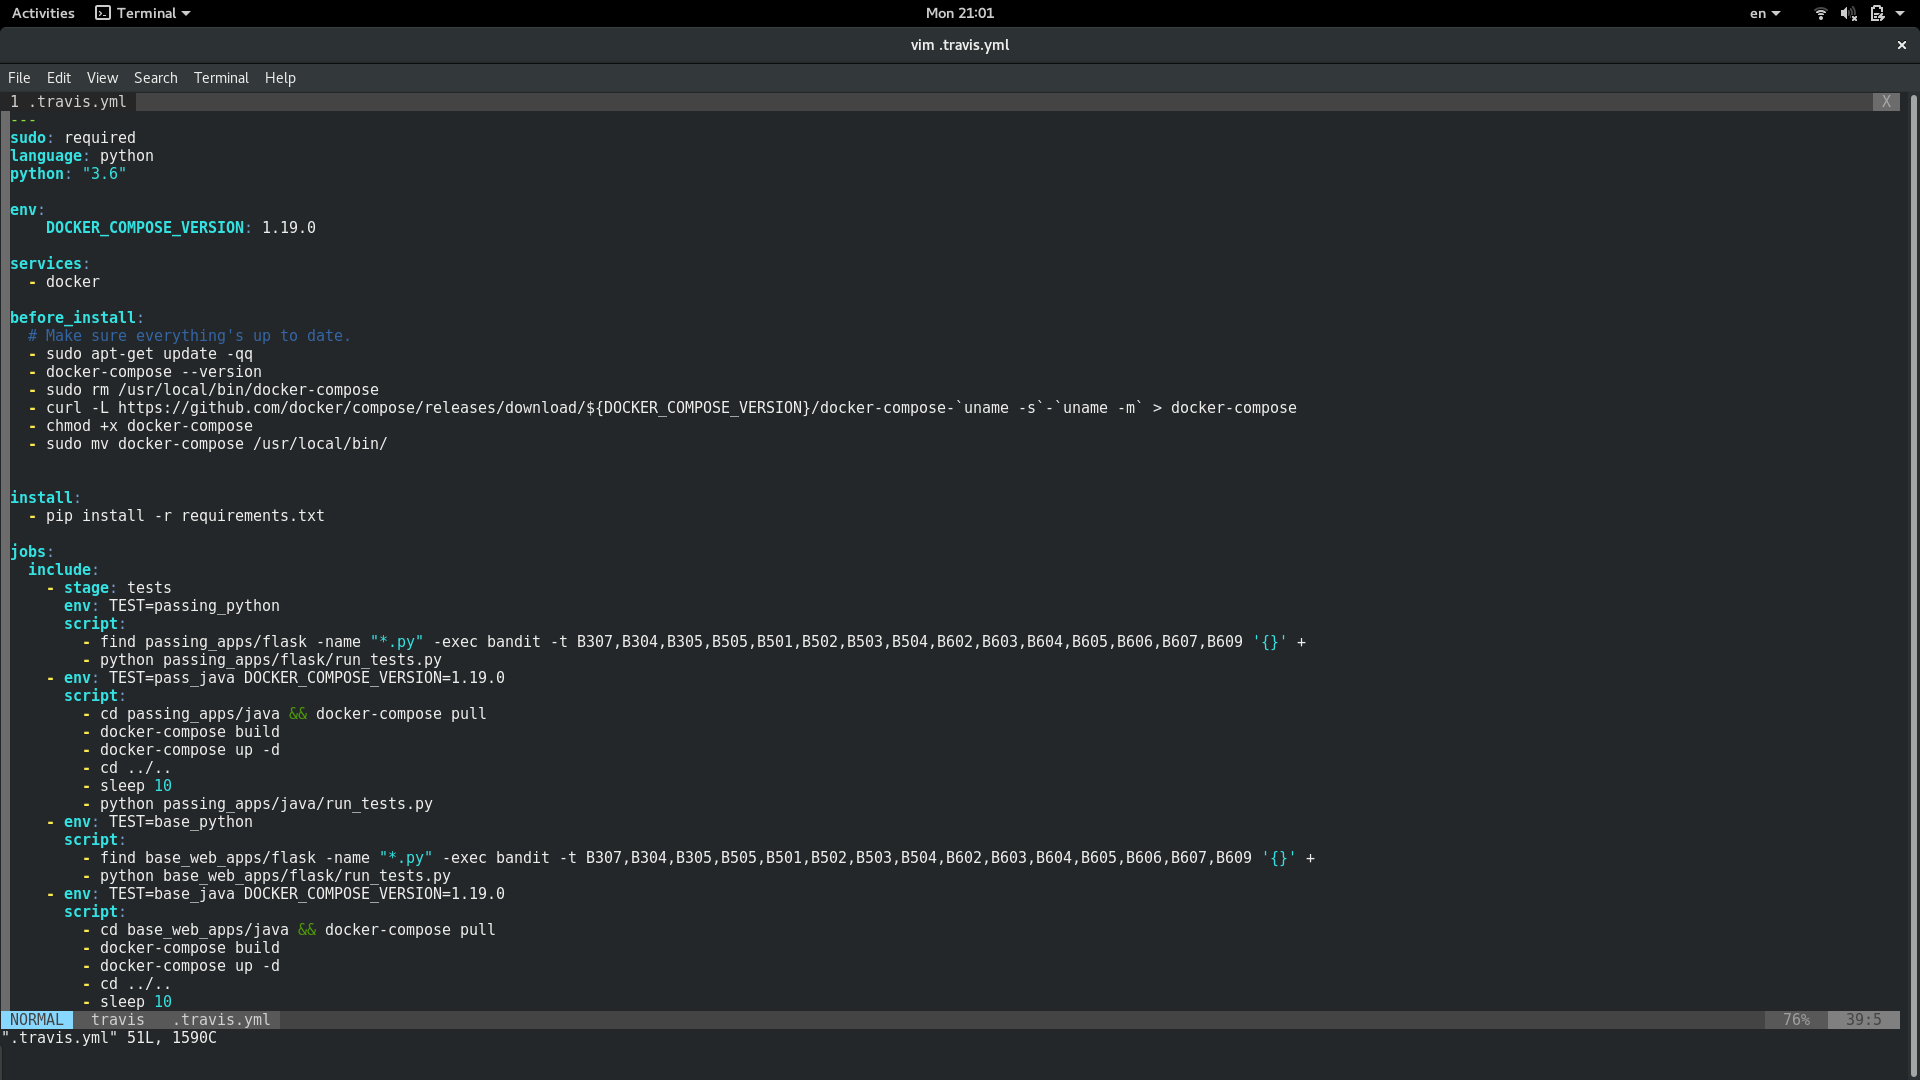
\includegraphics[width=6in]{travis}
\caption{\label{fig:fig4}}The travis configuration file
\end{figure}
The configuration involved install steps that installed docker-compose. This is required for running the dynamic tests against java, since it cannot just hook into the internal testing tools like
with flask. There are also settings for what version of python this project uses, that sudo is required, and docker needs to be installed. Then the stages are defined. There are two stages for python
and two for java. The TEST environment variables are set for visibility into what each build is doing from the travis webpage. In both python builds, first bandit is run against it with the tests
that address the use of subprocess, os, and crypto. Next the unit tests are run against the flask. For the java, first docker is set up and then the unit tests are run against them. If any of the
static tests trigger or the unit tests fail, then the entire build will fail. Figure~\ref{fig:fig5} shows an example of the builds being ran in travis.
\begin{figure}[!ht]
  \centering
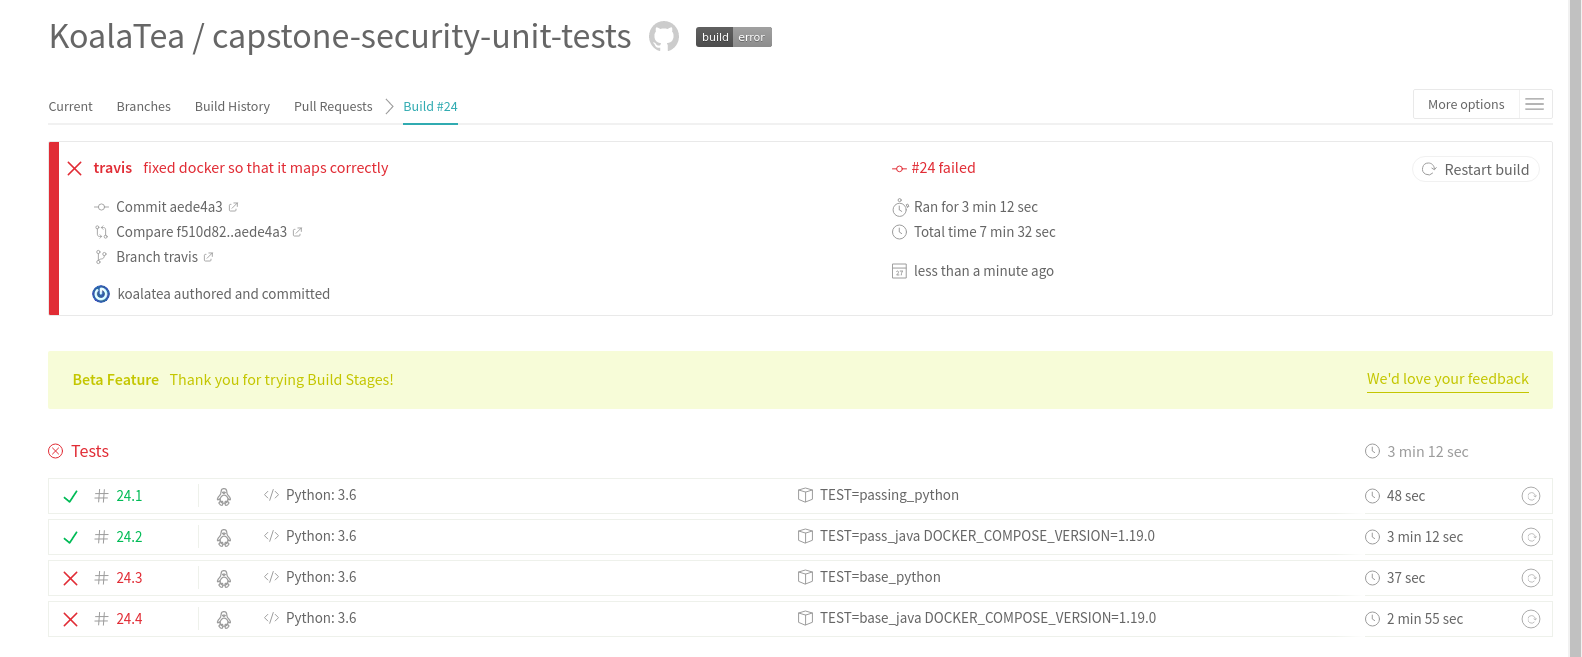
\includegraphics[width=6in]{travisbuilds}
\caption{\label{fig:fig5}}Builds being ran in travis
\end{figure}


\section{Testing and Experiments}
In this section, describe your testing and experiment design and setup, and conduct the testing and experiments, and generate data. 

Need to explain why your experiment design will do what is supposed to do, and describe the expected the result, and how the result may validate your ideas and/or support your project. 
\section{Data Analysis}

Based on the data generated from the testing and experiments, we derived the following results. The global temperature is increasing at an alarming rate as illustrated in Figure~\ref{fig:fig4}.  It is not real data, it is for demonstration only. 

  \begin{figure}[!ht]
 \centering
 
 
\begin{tikzpicture}[only marks, y=.5cm]
    \draw plot[mark=*,xshift=-6cm] file {ScatterPlotExampleData.txt};
    \draw[->,xshift=-6cm] (6,0) -- coordinate (x axis mid) (17,0);
    \draw[->,xshift=-6cm] (6,0) -- coordinate (y axis mid)(6,27);
    \foreach \x in {6,8,10,12,14,16}
        \draw [xshift=-6cm](\x cm,1pt) -- (\x cm,-3pt)
            node[anchor=north] {$\x$};
    \foreach \y/\ytext in {0/0,2.5/5000,5/10000,7.5/15000,10/20000,12.5/25000}
        \draw (1pt,\y cm) -- (-3pt,\y cm) node[anchor=east] {$\ytext$};
    \node[below=1cm] at (x axis mid) {Years};
    \node[left=2cm,rotate=90] at (y axis mid) {Temperatures};
\end{tikzpicture}

  \caption{\label{fig:fig4} Recent Global Temperature Data}
  
  \end{figure}
  
\section{Conclusions}
The project involved creating two applications that were mirrors of each other in functionality. The applications were created as tests were decided to create appropriate functionality for the tests.
One application was written in python with flask as the web framework, while the other one was written in java with spring as the web framework. Both applications had a home page and a page for
POSTing data to a form which would return success if the form was POSTed successfully and failed if it was not. This was all the functionality needed for the tests involved.
All applications were then dockerized. Then the tests were created, which lead to editing the base applications to also have a passing version. Finally the repository for this project was CI enabled
using travis which a travis-ci.yml file.
This was all to emulate a corporations environment, there would be an application hooked up to a CI pipeline. Every merge request to master would kick off a build job to run the tests and block on
failure of those jobs. The goal of this project in this environment is to efficiently mandate security configurations on web applications in this environment. This would ensure expected configurations
were in place and decrease attack surface of the application. To do so, the following is recommended when setting up a security focused pipeline.
\begin{itemize}
    \item Prioritize creating dynamic tests, these can be used across projects and language
    \item Create policies that outline the expected configuration based on the dynamic tests and mandate them across projects
    \item Create a method for containerizing all applications developed so that they can easily be tested with the dynamic tests
    \item Include a static analysis tool that focuses on security and the language the project is in into the pipeline
    \item If static tests are needed write them using the static analysis tool chosen
    \item Seperate the security pipeline from the normal unit test pipeline so that it is obvious whether the unit tests or the security pipeline failed 
\end{itemize}
Further work into this field could look into the rules around where to apply a security pipeline and how to have different levels besides just passing and failing builds. Another interesting field that
would be helpful to this pipeline is automatic test selection so that when a change is made to the code, only the tests that are relevant to that code are run. One more research topic could be looking
at how to use fuzzing effectively in a pipeline. All of these would be helpful to furthering the use of CI for security testing.

\section{Acknowledgment}
I thank my advisor for the guidance and I appreciate the financial support from my family and sponsors, .... 
\printbibliography




% ------------------------------------------------------------------------------
% End document
% ------------------------------------------------------------------------------
\end{document}
